\documentclass[11pt,a4paper,onecolumn,twoside]{mwart}

\usepackage[OT4]{fontenc}
\usepackage[cm]{fullpage}
\usepackage[pdftex,unicode=true]{hyperref}
\usepackage[polish]{babel}
\usepackage[utf8]{inputenc}
\usepackage{a4wide}
\usepackage{amsthm}
\usepackage{amsmath}
\usepackage{bm}
\usepackage{geometry}
\usepackage{graphicx,epstopdf}
\usepackage{icomma}
\usepackage{indentfirst}
\usepackage{polski}
\usepackage{titling}

\newtheorem{definition}{Definicja}
\newtheorem{axiom}{Aksjomat}

\begin{document}

\title{Modelowanie interferencji w komunikacji bezprzewodowej}
\author{Maciej Szeptuch}
\date{Wrocław, \today}
\maketitle

\abstract{\
    Głównym problemem wydajnej oraz bezawaryjnej komunikacji bezprzewodowej jest
    zapewnienie jakości połączenia między urządzeniami. Sygnał z nadajnika
    po drodze do odbiornika osłabia się oraz zniekształca. Odbiornik
    tak naprawdę nie słyszy oryginalnego sygnału tylko taki
    po zniekształceniach, na dodatek poskładany z innymi sygnałami otoczenia
    i zakłóceniami.
    \\
    Na przestrzeni lat powstało wiele modeli starających się opisywać
    komunikację bezprzewodową ale dopiero niedawno w szerszym użyciu zaczęły
    pojawiać się modele starające się brać pod uwagę to zjawisko (tzw.\
    interferencję). Uważane za najbardziej zbliżone do rzeczywistości, zazwyczaj
    też wykazane eksperymentalnie, są modele bazujące na formule SINR (signal to
    interference plus noise ratio). Niestety są one zarazem najbardziej
    skomplikowane z powodu będącej ich główną częścią asymetryczną, kumulatywną,
    wiele-do-jednego zależnością SINR\@. Dlatego też ciągle rozważane są
    prostsze modele starające się być z nią zgodne ale jednocześnie próbujące
    jak najlepiej ukryć bądź też pominąć skomplikowane jej części. Niestety
    prawie wszystkie z nich nie przedstawiają żadnych gwarancji na jakość
    wynikającej z uproszczeń aproksymacji.
    \\
    Przedstawię model SINR, kilka prostszych najpopularniejszych modeli które
    były do tej pory używane --- unit disk graphs (UDG), dual graphs, a także
    model conflict graphs i najnowszy wynik jego dotyczący, przedstawiony przez
    Halldorsson i Tonoyan, który nie tylko ściśle określa jego aproksymację
    względem SINR ale też dowodzi jej optymalności w kontekście abstrakcji
    grafowych.
}

\newpage

\section{Wstęp}
\subsection{Sieci bezprzewodowe}
Sieci bezprzewodowe stanowią nieodłączną część naszego życia, czy to komputery,
laptopy, smartfony, zegarki, czy też dowolne inne urządzenia (nawet żarówki,
lodówki), które za sprawą tzw.\ Internetu Rzeczy (ang. Internet of Things / IoT)
też zaczynają wymieniać się informacjami, w sercu każdego z nich jest zazwyczaj
jakaś sieć bezprzewodowa. W każdym domu znajduje się już co najmniej parę tego
typu urządzeń i muszą one jakoś się ze sobą skutecznie komunikować. Mimo ich
wszechobecności niewielu ludzi zdaje sobie sprawę z tego jak skomplikowanym
zadaniem jest zapewnienie ich jakości, niezawodności. Głównym problemem jest
tzw.\ interferencja, która występuje w momencie gdy wiele urządzeń próbuje się
komunikować w tym samym momencie, tak jak kiedyś --- na początku sieci kablowych
gdy cała komunikacja odbywała się w jednym współdzielonym kablu koncentrycznym
(zanim przeszliśmy na model switchowania i skrętkę), tak i tu wymusza ona
stosowanie zaawansowanych technik wyboru które połączenia są dozwolone tak aby
zapewnić maksymalne wykorzystanie dostępnego pasma przy niezawodności
odbywającej się komunikacji. Główną różnicą względem starych systemów jest to,
że teraz naszym medium jest trójwymiarowa przestrzeń --- powietrze, zamiast
dawnego jednowymiarowego kabla koncentrycznego na którym wszystko było prostsze.

\subsection{Interferencja}
W momencie kiedy wiele urządzeń na raz korzysta z tego samego kanału
komunikacyjnego, odbierane przez nie sygnały stają się złożeniem wszystkich
nadawanych transmisji, a także szumu i innych zakłóceń. Ale każde z nich chce
usłyszeć tylko jeden konkretny sygnał a nie miks wszystkiego co słychać wkoło
nich. To jest właśnie interferencja. Istnieją zaawansowane algorytmy, a także
specjalizowane układy pozwalające na rozdzielenie tych sygnałów umożliwiające
urządzeniom próbę odebrania transmisji która go interesuje ale nie są one
perfekcyjne. Gdy zakłócenia stają się stosunkowo duże to nic z takim sygnałem
nie da się już zrobić. Dlatego staramy się dążyć do ich redukcji, zazwyczaj
poprzez ograniczanie symultanicznie nadających urządzeń, dzieląc je na podzbiory
które mogą się komunikować w tym samym czasie, oczywiście wiąże się to ze
zmniejszeniem przepustowości sieci, więc dochodzimy do tak naprawdę zadania
optymalizacyjnego balansując pomiędzy niezawodnością komunikacji a jej
wydajnością.

\subsection{Szeregowanie połączeń}
Minimalizacja interferencji nie jest prostym zadaniem. W tym celu można
zarządzać mocą nadajników, aby sygnał był słyszany tylko tam gdzie potrzeba
i wprowadzał jak najmniej zakłóceń do całego systemu. Ale to podejście bardzo
szybko pokazuje swoje ograniczenia --- nie można zmniejszać mocy
w nieskończoność, w pewnym momencie nawet odbiornik nie będzie w stanie usłyszeć
nadawanych do niego komunikatów. Z tego powodu znacznie bardziej obiecującą
praktyką jest szeregowanie połączeń. Polega ono na takim wybieraniu transmisji
aby te odbywające się w tym samym momencie nie przeszkadzały sobie nawzajem
i pozwalały na skuteczną oraz wydajną komunikację wszystkich uczestniczących.
W celu określania optymalnych ustawień bierze się pod uwagę wszelkie możliwe
czynniki --- pozycje urządzeń w przestrzeni, ich moce nadawania, moce
wzmacniaczy odbiorników, przeszkody na drodze sygnału itp. Wszystko to składa
się na skomplikowane algorytmy mające na celu optymalizować wykorzystanie
medium komunikacyjnego.

\subsection{Modele}
Rzeczywistość jest dosyć skomplikowana, z tego powodu w celu uproszczenia
rozumowań, poszukuje się prostych abstrakcji skomplikowanych procesów.
Przykładem jest chociażby właśnie komunikacja bezprzewodowa. Cały czas poszukuje
się lepszych modeli przez zastosowanie prostszych, lepiej poznanych abstrakcji.
Najbardziej przystępną jest reprezentacja grafowa, znajduje ona zastosowanie
w bardzo wielu dziedzinach dzięki czemu jest bardzo dobrze zbadana i znamy wiele
jej własności. Ponadto wydaje się ona dosyć naturalna, urządzenia możemy
reprezentować przez wierzchołki a ich połączenia przez krawędzie. W porównaniu
do formuły SINR, która mimo tego że pozwala bardzo dokładnie reprezentować
rzeczywiste zachowanie sieci, jest niestety specyficzna, skomplikowana przez
co bardzo trudno z niej korzystać a co dopiero przedstawić ją w języku grafów.
Istnieje wiele prób przedstawiania komunikacji bezprzewodowej za pomocą grafów,
np.\ Disk Graphs --- szczegółowiej przy
założeniu o stałej mocy wszystkich nadajników --- Unit Disk
Graphs~\cite{Kuhn:2003:ANB:941079.941089}, w których przyjmuje się że każde
urządzenie ma pewien zasięg, który wystarcza do określenia czy dwa urządzenia
potrafią usłyszeć się nawzajem. Nowsze podejście starające się jakoś uchwycić
zawodność sieci tzw.\ Dual Graphs~\cite{Kuhn:2010:BUR:1835698.1835779} ---
przedstawia sieć jako dwa grafy, które mają wspólne wierzchołki ale różnią się
zbiorem krawędzi --- pierwszy zawiera tylko niezawodne krawędzie, natomiast
w drugim pojawiają się także krawędzie zawodne, które starają się jakoś
wyabstrahować skomplikowane zależności powodujące niepowodzenia w transmisjach.
Modelem z najbardziej obiecującymi wynikami są tzw.\ Conflict
Graphs~\cite{Halldorsson:2015:WGR:2746539.2746585} --- w których to na podstawie
żądanych połączeń tworzymy graf łączący te, które nie mogą być jednocześnie
wykonane i ograniczamy go z góry i z dołu poprzez specyficzną podklasę tych
grafów, która pozwala nam ściśle określić jego zależność względem SINR\@.

\section{SINR}\label{section:SINR}
\subsection{Opis}
Model SINR, często nazywany też fizycznym modelem, jest uważany za najbardziej
zbliżony do realiów. Model ten po pierwsze zakłada, że moc sygnału słabnie
wraz z odległością --- w najprostszym przypadku zazwyczaj przyjmuje się, że jest
równa nadawanej mocy podzielonej przez odległość pomiędzy nadajnikiem
a odbiornikiem do pewnej potęgi zależnej od warunków otoczenia. A po drugie
przyjmuje, że sygnały się kumulują. Transmisja jest uznana za poprawnie
zrealizowaną wtedy i tylko wtedy, gdy moc sygnału dostarczona do odbiornika
przez odpowiadający mu nadajnik jest co najmniej pewną stałą razy większa niż
suma wszystkich pozostałych sygnałów i szumu otoczenia. \\
Aby opisać model trochę dokładniej przyda się pare oznaczeń. Konkretniej,
niech \\
\\
\indent $s_i$, $r_j$ oznaczają odpowiednio $i$-ty nadajnik i $j$-ty odbiornik,\\
\indent $d_{i,j} = d(s_i, r_j)$ to odległość pomiędzy odpowiednim odbiornikiem
i nadajnikiem, \\
\indent $P(s_i)$ --- moc nadawanego sygnału przez $i$-ty nadajnik,\\
\indent a $N$ to szum otoczenia. \\
\\
Wtedy możemy powiedzieć, że współczynnik SINR dla $i$-tego odbiornika (czy też
$i$-tego połączenia) spełnia równanie

$$
SINR_i = \frac{P(s_i) \cdot d_{i,i}^{-\alpha}}{N + \sum_{j \neq i} P(s_j)
       \cdot d_{j, i}^{-\alpha}}
$$

gdzie $\alpha$ --- zazwyczaj $2 \le \alpha \leq 6$ --- oznacza współczynnik
utraty sygnału. Czyli moc sygnału dostarczona do odbiornika
($P(s_i) \cdot d_{i,i}^{-\alpha}$) przez sumę pozostałych sygnałów
odbieranych przez odbiornik i szumu otoczenia ($N + \sum_{j \neq i} P(s_j) \cdot
d_{j, i}^{-\alpha}$). \\
Wtedy też, przy $\beta$ --- współczynnik odbioru sygnału zależny od sprzętu,
sygnał zostanie poprawnie zdekodowany, odebrany wtedy i tylko wtedy, gdy

$$
    SINR_i \geq \beta
$$

co dokładnie oznacza, że sygnał od odpowiadającego nadajnika (tego którego
chcemy usłyszeć) jest co najmniej pewną stałą ($\beta$) razy mocniejszy niż
pozostałe słyszane sygnały. \\
Mówimy, że dany zbiór połączeń jest spełnialny jeśli wszystkie jego transmisje
się powiodą.

\begin{center}
    \begin{figure}[!ht]
        \begin{center}
            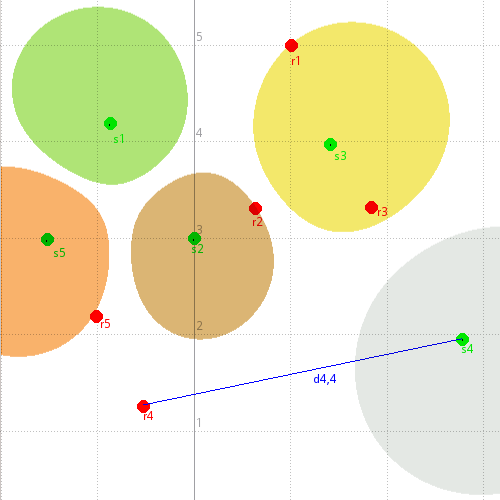
\includegraphics[width=0.5\textwidth]{pictures/model.png}
            \caption{Przykładowa wizualizacja modelu SINR, kolorowe pola to
                    obszary zasięgu odpowiadających im nadajników (zielonych
                    punktów)}
        \end{center}
    \end{figure}
\end{center}

\subsection{Zastosowania}
Większość prac wykorzystująca model SINR~\cite{Gupta:2006:CWN:2263214.2266070,
Moscibroda06thecomplexity} zazwyczaj zakłada geometryczne tłumienie
sygnału: utrata sygnału jest proporcjonalna do pewnego wielomianu odległości.
Podczas gdy to założenie jest prawdziwe w próżni, eksperymenty
wykazały~\cite{Baccour:2012:RLQ:2240116.2240123}, że rzeczywiste środowiska
są niestety znacznie bardziej skomplikowane. W rzeczywistości sygnał odbija się
od ziemi, ścian, różnych innych przeszkód na swojej drodze, przez co docierając
do odbiornika nie jest tylko  złożony z szumem i innymi sygnałami ale także
z samym sobą po pewnych przekształceniach, nie wspominając o różnych
przekształceniach pozostałych sygnałów. W szczególności jeśli spojrzymy na
standardowe zastosowania --- miasta czy mieszkania, gęstość występowania
wszelakich przeszkód jest stosunkowo duża (ściany, budynki itp.).
Eksperymentalne doświadczenia w takich środowiskach pokazały, że przyjęte
założenia odnośnie osłabienia sygnału ze wzrostem odległości są bardzo dalekie
od realów. W związku z tym podejmowane są próby użycia modeli bazujących na
pomiarach w konkretnym otoczeniu~\cite{Reis:2006:MMD:1151659.1159921,
DBLP:journals/corr/GudmundsdottirABFHJUV14}, zamiast tych bazujących na
teoretycznych geometrycznych założeniach. Problem jaki się niestety wtedy
pojawia jest taki, że już dosyć skomplikowane modele stają się jeszcze bardziej
skomplikowane poprzez to, że np.\ dla każdego połączenia musimy brać pod uwagę
jego unikalne pomiary. Wszystko to sprawia, że modele bazujące na SINR są dosyć
skomplikowane w badaniach i nadal poszukuje się lepszych sposobów na
przedstawianie interferencji.

\section{Unit Disk Graphs}
\subsection{Opis}
Jeden z dotychczas najpopularniejszych wśród teoretyków modeli, głównie ze
względu na swoją prostotę i podstawową, zadowalającą zgodność z rzeczywistością.
W tym wariancie zakłada się, że wszystkie urządzenia nadają z tą samą mocą. Ich
zasięg jest więc reprezentowany przez pewien stały promień. To pozwala określić
największy zbiór możliwych połączeń, do tego dołącza się jeszcze na przykład
własność, że odbiornik ma szanse usłyszeć odpowiadający mu nadajnik wtedy
i tylko wtedy, gdy żaden inny z jego sąsiadów nie nadaje. Z jednej strony jest
to oczywiście ogromne uproszczenie rzeczywistości, nie bierze pod uwagę
odległych interferencji, czy innych warunków otoczenia oprócz
odległości. Z drugiej jednak strony model jest na tyle przystępny, że pozwala na
uzyskiwanie silnych teoretycznych wyników~\cite{Alzoubi:2002:MCD:513800.513820,
Kuhn:2002:AOG:570810.570814}.

\subsection{Zastosowania}
Dzięki swojej przystępności i prostocie model UDG jest bardzo popularny,
szczególnie uwidacznia się to w badaniach tzw.\ sieci Ad-Hoc, w których można
na niego trafić bardzo często. Prawdopodobnie popularność UDG wynika także
z tego że modelowanie sieci Ad-Hoc korzystając z SINR jest zdecydowanie bardziej
skomplikowane. W sieciach tego typu każde urządzenie samo reguluje swój dostęp
do sieci na podstawie swojego lokalnego otoczenia, w przeciwieństwie do
standardowo stosowanego rozwiązania infrastruktury (ang.\ managed), w którym
jedno, centralne urządzenie steruje tak naprawdę całym przepływem informacji.
Takie podejście sprawia, że w SINR trzeba skrupulatnie brać pod uwagę każde
obecne urządzenie, które może wprowadzać interferencje, gdzie w sieci
zarządzanej można upraszczać środowisko zakładając, że nadzorca pozwala
odpowiednio dobierać jednocześnie komunikujące się urządzenia. W sieciach Ad-Hoc
widać, że modele typu UDG gdzie te zależności są uproszczone do grafu
(i na dodatek pomija się kwestię szumów itp.) są bardziej przystępne w analizie
niż np.\ model fizyczny. Niestety nie ma też specjalnie badań w kierunku
wykazywania jak te modele mają się np.\ do SINR, w efekcie nie ma możliwości
ustalenia z jaką dokładnością potrafią one przybliżać rzeczywistość
(poza eksperymentami oczywiście). Sprawia to, że wyniki są co prawda bardzo
obiecujące ale niespecjalnie przekładają się na praktyczne wnioski,
zastosowania.

\section{Dual Graphs}
\subsection{Opis}
Nowsze podejście starające się jakoś uchwycić zawodność sieci, tzw.\ Dual
Graphs~\cite{Kuhn:2010:BUR:1835698.1835779}, przedstawia sieć jako parę grafów,
które mają wspólne wierzchołki ale różnią się zbiorem krawędzi. Pierwszy graf
zawiera tylko niezawodne krawędzie, na których komunikacja zawsze się powodzi,
natomiast w drugim pojawiają się także krawędzie zawodne, które mają
wyabstrahować skomplikowane zależności powodujące niepowodzenia w transmisjach.
Zawodność jest tu kontrolowana przez adwersarza. Po pierwsze wybiera on na
których zawodnych krawędziach przesłanie wiadomości się powiodło. Po drugie,
jeśli do wierzchołka dotrze wiele wiadomości, on może wybrać czy powstała
kolizja, czy też jedna z wiadomości została usłyszana.

\subsection{Zastosowania}
Większość stosowanych grafowych modeli zazwyczaj zakłada, że dla ustalonego
grafu komunikacja po jego krawędziach jest niezawodna. Nie jest to specjalnie
zgodne z rzeczywistością ale na pewno sprawia, że analiza takich modeli jest
prostsza i pozwala na formułowanie mocniejszych hipotez. Poprzednie podejścia
do osłabienia tych założeń (jak na przykład~\cite{Kuhn:2003:ANB:941079.941089})
sukcesywnie zacierały tę granicę. Model Dual Graphs za to pozwala teoretycznie
pozbyć jej się całkowicie. W przeciwieństwie do innych modeli Dual Graphs
uwzględnia fakt, że komunikacja nie jest niezawodna. Wykorzystanie do tego celu
drugiego grafu krawędzi zawodnych sprawia też, że wydaje się on przystępny dla
prób rozszerzania poprzednich algorytmów budowanych tylko dla grafu komunikacji.
Niestety w praktyce tego jeszcze nie widać, nie ma wiele prac starających się
wykorzystać model Dual Graphs ale na pewno wydaje się on bliższy rzeczywistości
od poprzedników. Nadal jednak nie ma też specjalnie badań na temat zgodności
algorytmów wykorzystujących ten model z rzeczywistością. Sprawia to, że też
ciężko określić jak bardzo model Dual Graphs może być przydatny w praktycznych
zastosowaniach.

\section{Conflict Graphs}
\subsection{Opis}
Modelem stosunkowo dobrze odzwierciedlającym rzeczywistość są tzw.\ Grafy
Konfliktu (ang.\ Conflict Graphs) --- w których to na podstawie żądanych
połączeń tworzymy graf łączący krawędziami te, które nie mogą być jednocześnie
wykonane. W najnowszym wyniku~\cite{Halldorsson:2015:WGR:2746539.2746585}
Halldorsson i Tonoyan pokazują jak ograniczyć możliwą reprezentację grafu
konfliktu dla zadanego zbioru połączeń poprzez specyficzną podklasę tych grafów,
która pozwala ściśle określić jego zależność względem SINR\@.
Mając taki graf wystarczy go na przykład pokolorować aby dostać zbiory
niezależnych połączeń, które wykonywane jednocześnie nie powinny się nawzajem
zakłócać.

\subsection{Szczegóły}
Aby graf mógł być nazywany grafem konfliktu powinien spełniać pewne założenia.
W celu znormalizowania reprezentacji połączeń za pomocą grafu konfliktu stosuje
się pięć opisanych poniżej aksjomatów.

\begin{axiom}
    Graf konfliktu jest zdefiniowany przez wzajemne relacje na połączeniach.
\end{axiom}
Konkretniej, oczekujemy, że istnienie krawędzi pomiędzy połączeniami $i$
oraz $j$ zależy tylko od właściwości tych dwóch połączeń, bez wpływu żadnego
z pozostałych.

\begin{axiom}
    Graf konfliktu jest niezależny od pozycji i skali rzeczywistych połączeń.
    Przesunięcie bądź powiększenie przez stały czynnik nie wpływa na relacje
    konfliktu (istnienie krawędzi) połączeń.
\end{axiom}
To wynika z SINR, jest ona tak sformułowana, że opiera się tylko na względnej
odległości pomiędzy urządzeniami a nie ich rzeczywistymi pozycjami. Oczywiście
istnieje limit na długość połączenia wynikający z obecności niezależnego szumu
otoczenia ale przeszkadza on tylko w specyficznych przypadkach, jest więc
pomijany.

\begin{axiom}
    Relacja konfliktu jest monotoniczna ze wzrostem odległości.
\end{axiom}
Dokładniej mamy na myśli to, że jeśli dwa połączenia są w konflikcie
to zmniejszenie odległości między nimi nie neguje tej relacji. Podobnie jeśli
dwa połączenia nie są w konflikcie to zwiększenie odległości pomiędzy nimi
też nic nie zmienia.

\begin{axiom}
    Graf konfliktu powinien reprezentować niekompatybilność połączeń.
\end{axiom}
Aksjomat ten oznacza, że jeśli dwa połączenia nie mogą współistnieć w jednym
rozwiązaniu, muszą być połączone krawędzią w grafie konfliktu.

\begin{axiom}
    W przypadku dowolnej regulacji mocy, graf konfliktu jest symetryczny ze
    względu na rozróżnienie nadajników
    i odbiorników.
\end{axiom}
Szczegółowiej, nie powinno mieć znaczenia, które z końców połączeń nadają,
a które słuchają w przypadku określania czy dwa połączenia kolidują ze sobą. \\
\\
Te pięć aksjomatów implikuje własność, że tylko dwie odległości mają znaczenie
przy formułowaniu konfliktów: długość dłuższego połączenia oraz odległość
pomiędzy nimi (definiowana przez najkrótszą z czterech odległości pomiędzy
końcami), obydwie przeskalowane przez długość krótszego połączenia. \\
\\
Dla tak zdefiniowanych grafów konfliktu można się zastanowić jak ograniczyć
tę reprezentację tak aby miała ona coś wspólnego z SINR\@. W tym celu po
pierwsze definiuje się \textit{f-niezależność} tj.\

\begin{definition}
    Dla dodatniej, niemalejącej podliniowej funkcji $f$ dwa połączenia $i$,$j$
    nazwiemy \textit{f-niezależnymi} jeśli
    $$
    \frac{d(i,j)}{d_{\min}} > f\left(\frac{d_{\max}}{d_{\min}}\right)
    $$
    gdzie $d_{\min} = \min(d_{i,i},d_{j,j})$, $d_{\max} = \max(d_{i,i},d_{j,j})$
    i w przeciwnym wypadku są \textit{f-sąsiadujące}.\footnote{oznaczenia
    odległości z modelu SINR przedstawionego w punkcie~\ref{section:SINR}} \\
    Zbiór połączeń jest \textit{f-niezależny} (\textit{f-sąsiadujący}) jeśli
    wszystkie połączenia są parami \textit{f-niezależne}
    (\textit{f-sąsiadujące}).
\end{definition}

Korzystając z \textit{f-niezależności} definiujemy graf konfliktu
$\mathcal{G}_f$ taki, że dwa wierzchołki są połączone krawędzią wtedy i tylko
wtedy, gdy są \textit{f-sąsiadujące}. \\
\\
Wykorzystując \textit{f-niezależność} oraz aksjomaty można pokazać,
że dowolny graf konfliktu można reprezentować za pomocą $\mathcal{G}_f$
z dokładnością do pewnej stałej $\gamma \geq 1$ tj.\ dla dowolnego grafu
konfliktu $\mathcal{K}$ zachodzi $\mathcal{G}_f \subseteq \mathcal{K} \subseteq
\mathcal{G}_{\gamma f}$.
\\\\
Mając już znormalizowany sposób reprezentacji dowolnego grafu konfliktu wypada
jeszcze pokazać, że rozbieżność wynikająca ze stałej $\gamma$ nie wpływa
znacząco na strukturę tego grafu. W efekcie pokazuje się, że liczby chromatyczne
ograniczających grafów różnią się stałym współczynnikiem (konkretniej dla
$\gamma > 0$ zachodzi $\chi\left(G_{f}\right) =
\Theta\left(\chi\left(G_{\gamma f}\right)\right)$. \\
\\
Ostatnim najważniejszym krokiem jest pokazanie, że spełnialność według SINR
zawiera się pomiędzy $\mathcal{G}_{\gamma}$ oraz $\mathcal{G}_f$ dla odpowiednio
dobranej funkcji $f$ tj.\ każdy spełnialny zbiór jest niezależny w
$\mathcal{G}_{\gamma}$ oraz każdy niezależny zbiór z $\mathcal{G}_f$ jest
spełnialny. \\
\\
Teraz jak już mamy ograniczenie reprezentacji grafu konfliktu dla instancji SINR
(z akapitu wyżej), trzeba jeszcze zwrócić uwagę na wynikającą z niego dodatkową
rozbieżność. W tym celu pokazuje się, że liczby chromatyczne ograniczających
grafów różnią się praktycznie co najwyżej o stałą (konkretniej
$O(f^{*}(\Delta))$, gdzie $\Delta$ to stosunek najdłuższego do najkrótszego
połączenia, a $f^{*}$ to iterowana funkcja $f$).
Na tej podstawie można wnioskować o sile tej aproksymacji bazując na liczbach
chromatycznych tych ograniczeń.
\\\\
W efekcie uzyskujemy ścisłe określenie jak ta klasa grafów potrafi aproksymować
zależność SINR\@. Po szczegółowe dowody przedstawionych przekształceń odsyłam do
oryginalnej pracy~\cite{Halldorsson:2015:WGR:2746539.2746585}, są one bardziej
techniczne niż odkrywcze --- w esencji polegają na odpowiednim dobraniu stałych
i przeprowadzeniu nieskomplikowanych przekształceń.

\section{Wnioski}
Autorzy pokazali, że podana przez nich reprezentacja grafowa pozwala zachowywać
własności SINR ze stałym współczynnikiem aproksymacji. Ponadto udowodnili, że
jest to najlepsza możliwa grafowa aproksymacja sieci SINR\@. W kontekście modeli
podali także silny argument przeciw możliwości istnienia aproksymacji dla
dowolnych metryk oraz aproksymacji względem liczby połączeń. Ponadto, pokazując
zarazem użyteczność tego modelu, pokazali także $O(\log^*\Delta)$-aproksymacje
dla problemu planowania z dowolnym sterowaniem mocą bazującą na nim.

\section{Podsumowanie}
Niniejsze opracowanie przedstawia najpopularniejsze modele stosowane do
obrazowania komunikacji bezprzewodowej oraz najnowszy, bardzo ciekawy wynik
dotyczący tego tematu. Przybliża model SINR, stara się pokazać jego problemy
oraz złożoność, a także pokazuje jak wyniki ostatnich badań pozwalają budować
grafowe modele, które można bezpośrednio do niego odnieść. W wielkim skrócie
streszcza także obiecujące rezultaty, które udało się uzyskać bazując na tych
nowych badaniach. Pozwala to mieć nadzieję na rozwój algorytmów, które nie tylko
przystępnie się analizuje, dzięki bazowemu modelowi grafowemu, ale także
efektywnie działają w rzeczywistych sieciach.

\bibliography{essay}{}
\bibliographystyle{plain}

\end{document}
